\section{Los datos y las expresiones de género}
En el experimento se inscribieron 113 estudiantes de pregrado, de 29 de las 39 carreras de la universidad,\footnote{La participación por facultades se distribuye de la siguiente manera: 44\% de de Ingeniería, 13\% de Arquitectura y Diseño, 12\% de Ciencias Sociales, 10\% de Ciencias, 7\% de Arte y Humanidades, 6\% de Economía, 5\% de Derecho y 2\% de Administración y la Escuela de Gobierno.} de los cuales 56 se identificaron de manera masculina, 56 de manera femenina y uno se identificó de manera no binaria. A continuación, son descritos los criterios utilizados para clasificar la vestimenta, las habilidades y las aspiraciones como expresiones de género y se comprueba si, bajo esa clasificación, los participantes cumplen la norma social de que las personas de identidad femenina en promedio tienen expresiones femeninas y las personas de identidad masculina tienen expresiones masculinas. Lo anterior es una aproximación a si los participantes perciben la vestimenta, la habilidad o la aspiración como expresiones de género o no.

\subsection{Vestimenta} La vestimenta es una expresión visual con una fuerte asociación al género. Para identificar una vestimenta que mejor se acercara a la expresión de género de la persona, cada participantes observaba en la encuesta nueva vestimentas (ver Figura \ref{fig:vestimentas}).\footnote{Estas imágenes aparecían en un orden aleatorio, diferente para cada participantes para evitar efectos de orden.} Los participantes debían elegir cuál de esas vestimentas usaría con mayor frecuencia para ir a la universidad.

\begin{figure}[htbp]
    \centering
    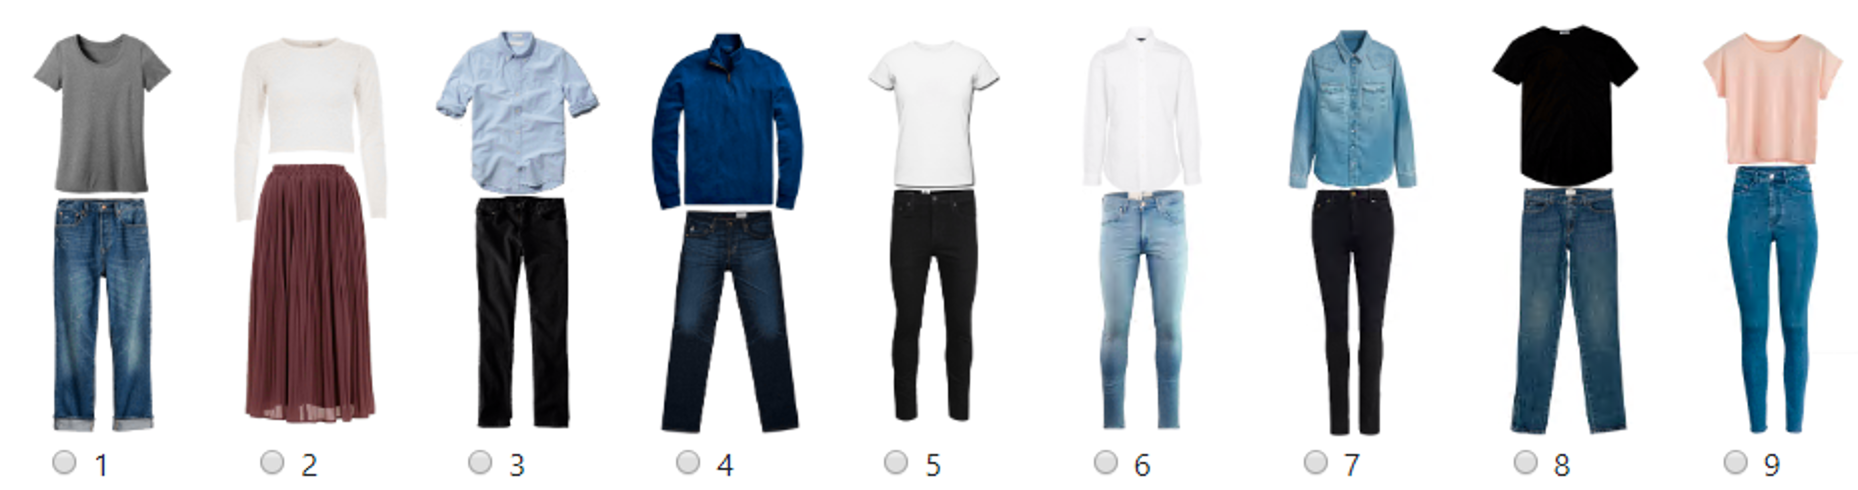
\includegraphics[width=14cm]{Images/vestimentas.png}
    \caption{Opciones de vestimentas a elegir}
    \label{fig:vestimentas}
    \begin{singlespace}
    \floatfoot{\footnotesize{\textit{Nota:} La figura contiene las opciones de vestimenta que observaban los participantes en la encuesta de inscripción. A cada persona le salía las vestimentas en un orden aleatorio y debían elegir la opción que consideraban usarían con mayor frecuencia para ir a la universidad.}\par}
    \end{singlespace}
\end{figure}

Las vestimentas fueron clasificadas como expresión de género masculina o femenina a partir de una encuesta de percepción hecha a una muestra de estudiantes diferente a la de los participantes, pero de la misma universidad. En esa encuesta, las personas debían responder de 1 a 9 qué tan masculina o femenina percibían esa vestimenta.\footnote{Para la mitad de los encuestados, 1 representaba muy femenina y para la otra mitad, 1 representaba muy masculina.} El puntaje promedio de cada vestimenta fue asignado a esta y luego, en la muestra de participantes, ese puntaje fue estandarizado. El puntaje estandarizado, que es creciente en la feminidad, es la medida de cada vestimenta como expresión de género. 

Entre los participantes, la elección de vestimentas es bimodal y está altamente relacionado con la identidad de género de los participantes (ver Figura \ref{fig:distribuciones_expresiones}; p-valor de la prueba Kolmogorov-Smirnov: 0.000). En promedio, el puntaje de la vestimenta que eligieron las personas de identidad masculina es de -0.81 (d.e 0.49) y el de las personas de identidad femenina es de 0.81 (d.e 0.64). Esto es indicativo de que los participantes sí perciben la vestimenta como expresión de género. 

\subsection{Habilidad} 
La habilidad es una aproximación a la norma social de que las mujeres son buenas comunicándose y los hombres son buenos para las matemáticas. Esta expresión de género es relevante en este caso dado que el experimento fue conducido en un ambiente universitario en el que existe una baja participación femenina en carreras intensivas en matemáticas y una baja participación masculina en carreras de ciencias sociales. Esta norma social y su persistencia a través de las generaciones ha sido ampliamente estudiado por la literatura \citep{nollenberger2016mathgap, giuliano2017gender, saltiel2019gendergapinSTEM, spencer1999mathgenderstereotype, cvencek2011mathgenderstereotype}.

\begin{figure}[htbp]
    \centering
    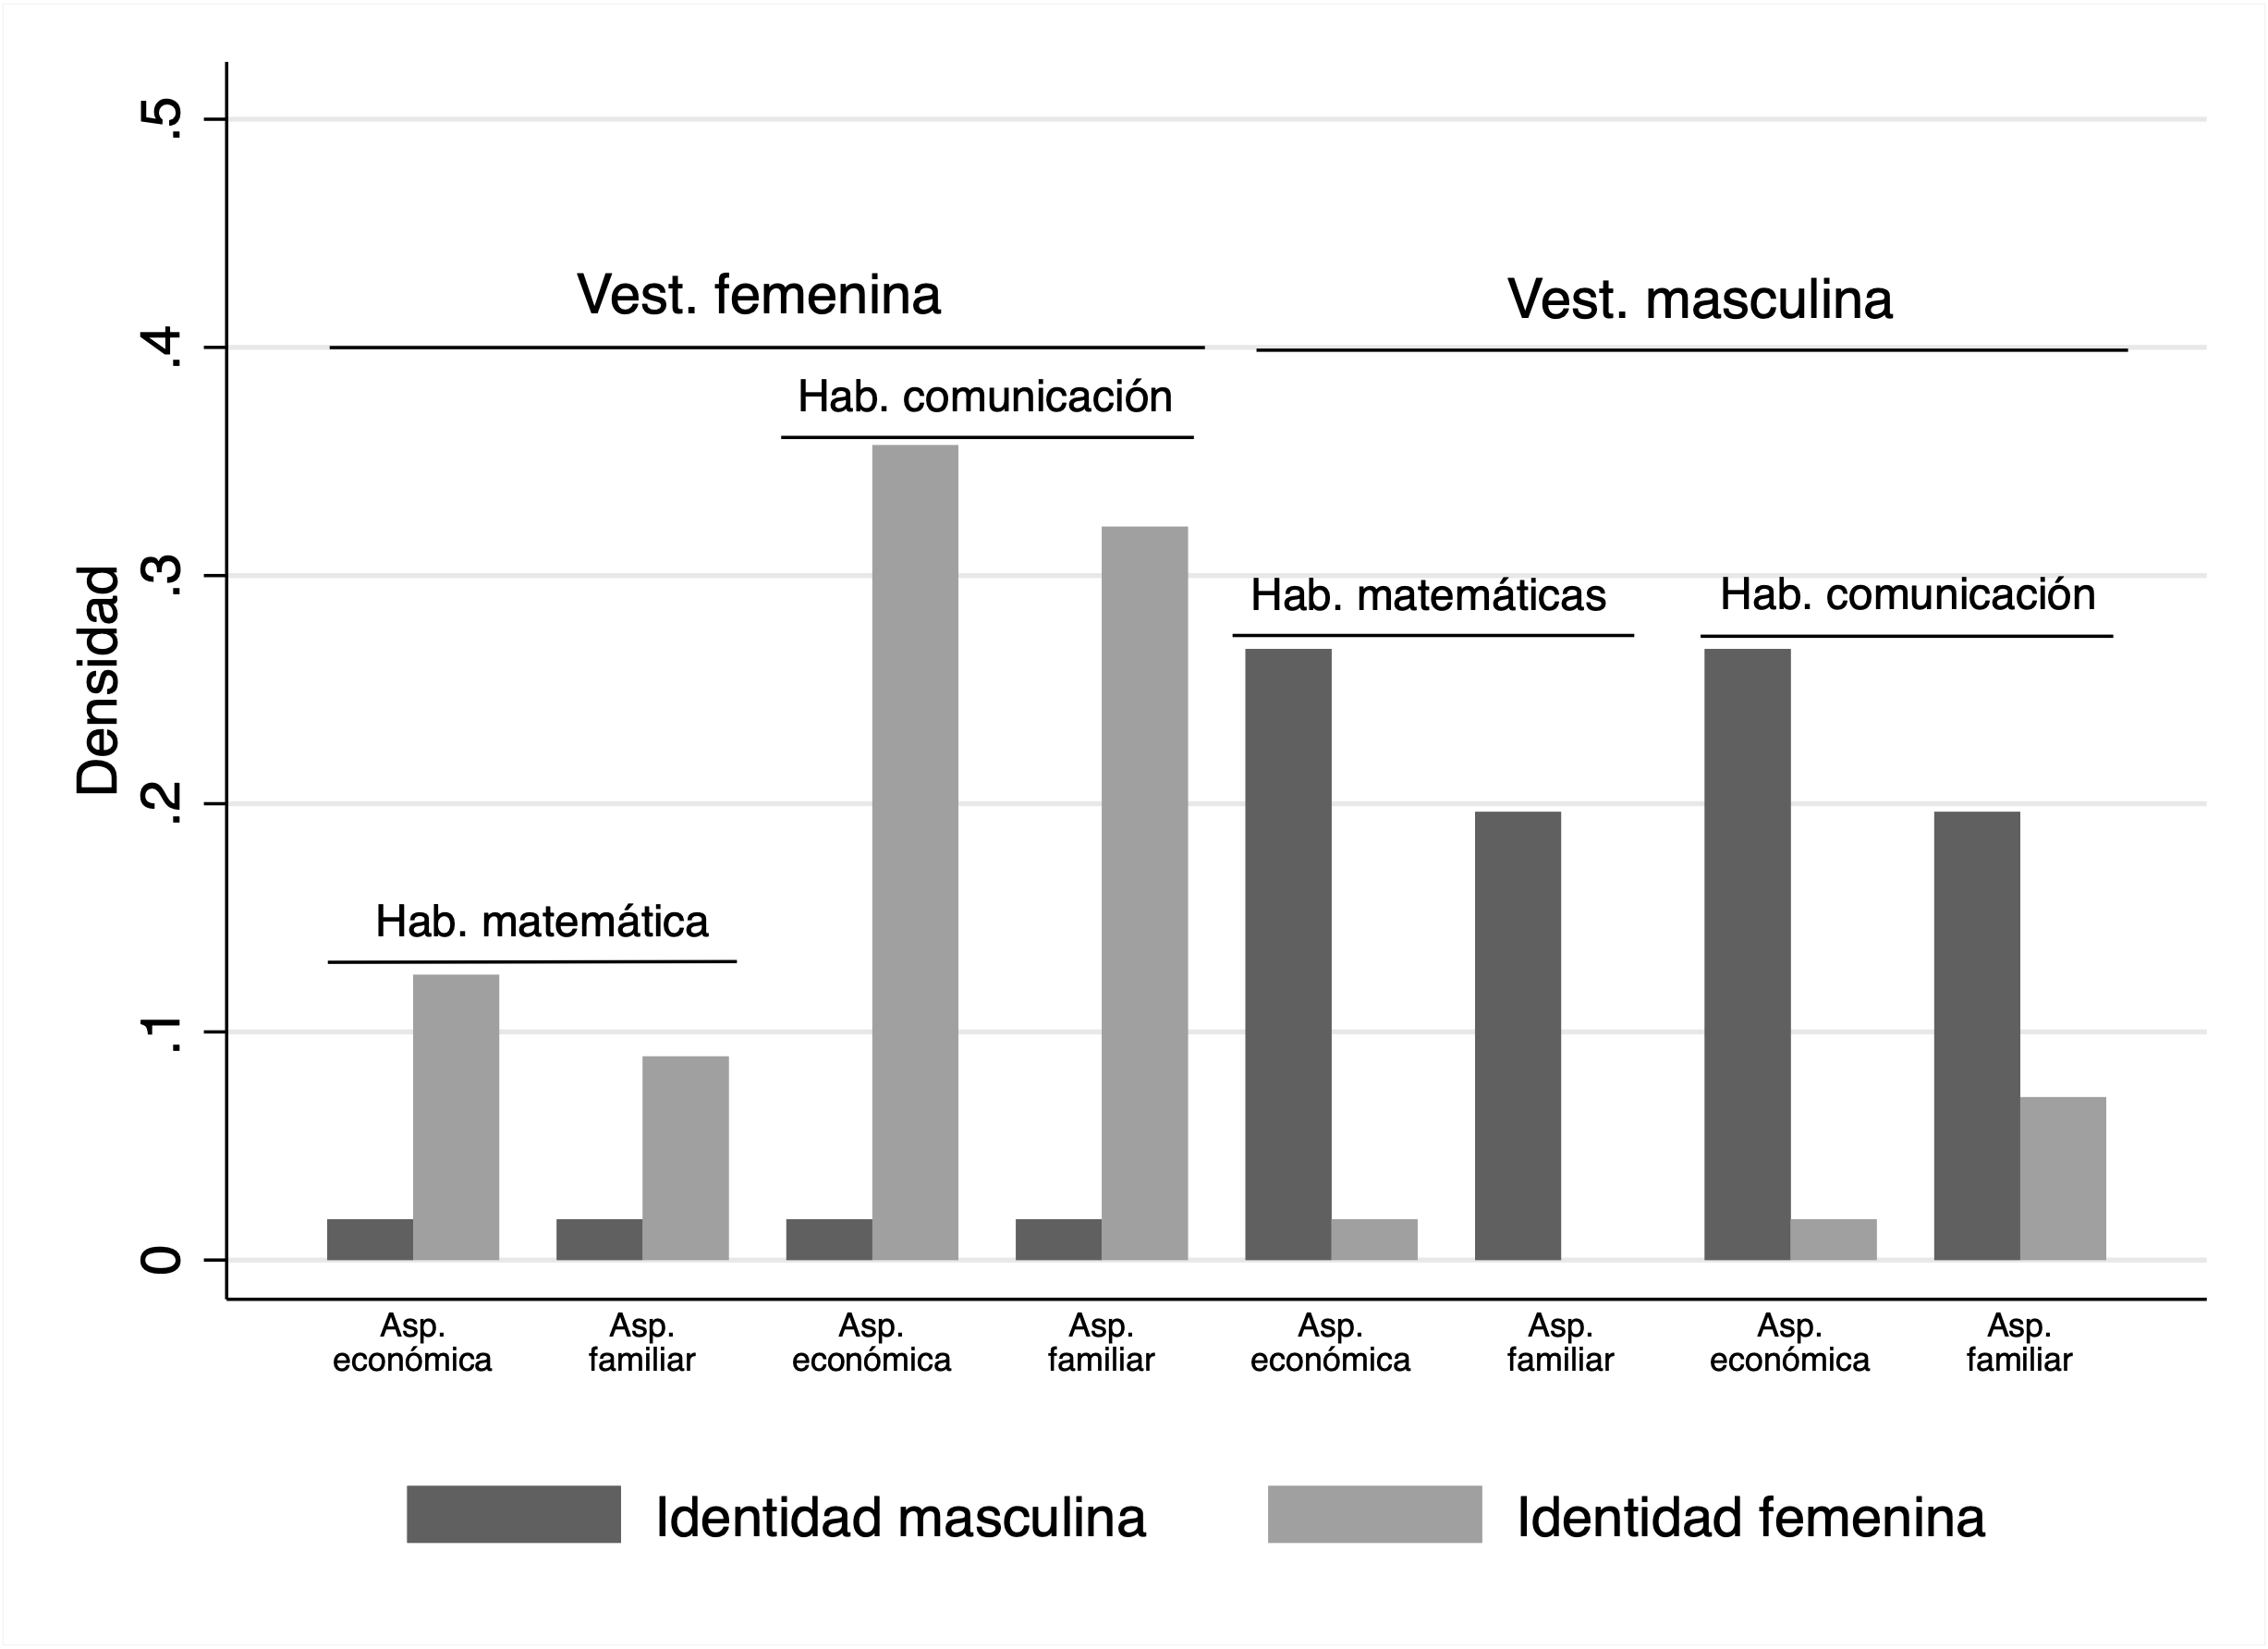
\includegraphics[width=11cm]{Images/dist.png}
    \caption{Distribución por género de vestimenta, habilidad y aspiración}
    \label{fig:distribuciones_expresiones}
    \begin{singlespace}
    \floatfoot{\footnotesize{\textit{Nota:} La figura representa la cantidad de participantes con esas características, discriminado por la identidad de género que reportó cada participante en la inscripción. Para esta gráfica, se definió una vestimenta femenina aquella que tenía un puntaje $>\ 0$ y una vestimenta masculina una con un puntaje $<\ 0$. El puntaje de la vestimenta es un puntaje estandarizado. La Tabla \ref{tab:distribuciones_expresiones} presenta esta información y contiene el número de observaciones por categoría.}\par}
    \end{singlespace}
\end{figure}

Además, en la encuesta de percepción hecha a una muestra diferente a la de los participantes, las personas respondieron de 1 a 9 qué tan masculina o femenina percibían 30 carreras universitarias. Al clasificar las carreras entre intensiva y no intensivas en matemáticas, la percepción de las personas que respondieron esta encuesta es que todas las carreras no intensivas en matemáticas son consideradas femeninas, en algún grado. Mientras que el 75\% de las carreras intensivas en matemática son consideradas masculinas. El 25\% de las carreras intensivas en matemáticas que no perciben masculinas, las perciben mínimamente femeninas -muy cerca al punto neutral- (ver Figura \ref{fig:careers}). Esta clasificación de las carreras valida la norma social que asocia las matemáticas con lo masculino y las comunicaciones con lo femenino.

Para identificar si los participantes creían ser más hábiles en matemáticas o en comunicación, la encuesta de entrada incluía una lista de ocho habilidades, entre las que estaban estas dos. Para cada habilidad, debían responder de 1 a 4 qué tan hábiles son. Luego debían responder con una escala de likert si consideraban ser mucho más hábiles en matemáticas o mucho más hábiles comunicándose. La encuesta incluía otra escala de likert, entre otras dos habilidades, para no hacer evidente cuáles eran las habilidades de interés. En la tarjeta, aparecía como habilidad principal comunicación (matemáticas) si le daban a esta un mayor puntaje que a matemáticas (comunicación). En caso de que le dieran el mismo puntaje, la habilidad principal era la que reportaran en la escala de likert como la más fuerte. Para aproximadamente el 97\% de la muestra, la habilidad definida con el puntaje es igual a la que reportaron en la escala de likert. 

Entre los participantes del experimento, existe una diferencia entre la habilidad que perciben más fuerte las personas femeninas que las masculinas (ver Figura \ref{fig:distribuciones_expresiones}; p-valor de prueba $\chi^2$: 0.003). Esta diferencia se debe a que el 76\% de las personas de identidad femenina considera ser mucho más hábiles comunicándose que en matemáticas. Mientras que las personas de identidad masculina se distribuyen en partes iguales entre aquellos que consideran ser más hábiles en matemáticas y los que consideran ser más hábiles comunicándose. Por lo que, al menos las personas de identidad femenina, sí perciben la habilidad como una expresión de género. 

\subsection{Aspiración principal} 
La aspiración principal busca identificar si en los próximos 10 años las personas aspiran más a tener una familia estable o tener mucha comodidad económica. La aspiración familiar es una aproximación a la norma social de que las mujeres se encargan del hogar y del cuidado de otros, mientras que los hombres son los proveedores económicos del hogar. Lo anterior siguiendo la literatura que ha estudiado la distribución de labores en el hogar, la carga de cuidado que asumen las mujeres \citep{floro1995gendertimeallocation, urdinola2017timeusegender}, la participación laboral en relación como la maternidad \citep{lundborg2017childrencareer}  y la distribución de ingresos al interior del hogar \citep{bertrand2015genderandincome, Robinson2012incomeallocationandshocks}, entre otros. 

Siguiendo la misma estructura utilizada para categorizar la habilidad principal,  los participantes debían responder para siete elementos, de 1 a 4,  qué tan importante es para ellos tener eso en los próximos 10 años. Entre esos siete elementos estaban estabilidad familiar y vivir muy cómodo económicamente. Luego debían responder dos escalas de likert sobre sus aspiraciones, una de ellas ponía en un extremo la comodidad económica y en el otro extremo la estabilidad familiar. En la tarjeta que caracterizaba a una persona aparecía una aspiración familiar (económica) si reportaba que era más importante en los próximos 10 años tener estabilidad familiar (comodidad económica) que comodidad económica (estabilidad familiar). En caso de que le dieran el mismo puntaje, la aspiración que aparecía en la tarjeta era la que reportaron que aspiran más en la escala de likert. Al igual que con la habilidad, en la mayoría de los casos la aspiración construida con la relación entre el puntaje que le dio a la estabilidad familiar y a la comodidad económica, coincidía con lo que reportó en la escala de likert. 

Entre los participantes no existe una diferencia clara entre la frecuencia de personas de identidad femenina y las de identidad masculina que aspiran más a tener estabilidad familiar ni las que aspiran más a tener comodidad económica (ver Tabla ver Figura \ref{fig:distribuciones_expresiones};  p-valor de la prueba $\chi^2$: 0.569). Esto es indicativo de que, para esta muestra, la aspiración no es percibida como una expresión de género. Por lo tanto, en adelante no se tomará en cuenta la aspiración como expresión de género. 

Existen varias posibilidades de por qué esta muestra no percibe la aspiración como expresión de género. Primero, puede existir un cambio generacional y diferencias contextuales. La literatura ha estudiado la división de trabajo en el hogar para una generación y un contexto diferente. Por lo que es posible, que la asociación familia- femenino, trabajo/recursos económicos-masculino se haya perdido. Segundo, puede que la asociación siga existiendo, pero no a nivel de aspiraciones. Es decir, una persona puede reconocer que la sociedad espera una mujer cuidadora y un hombre proveedor, pero que su aspiración sea ir más allá de lo que la sociedad espera. 

